\documentclass{my_paper}
\usepackage{ctex}
\usepackage[textwidth=444bp,vmargin=2.5cm]{geometry}%设置页边距
\usepackage{array} %主要是增加列样式选项
\usepackage[dvipsnames]{xcolor}%颜色宏包
\usepackage{graphicx}%图片宏包
\usepackage{amsmath}%公式宏包
\usepackage{amsthm}
\usepackage[T1]{fontenc}    
\usepackage{newtxtext, newtxmath}  %两种使用Times New Roman 字体的方法
\usepackage[english]{babel}
\usepackage{float}
\usepackage{algorithm}
\usepackage{algorithmic}
\newcommand{\R}{\mathbb{R}}
\newtheorem{theorem}{Theorem}
\newtheorem{corollary}{Corollary}[theorem]
\newtheorem{lemma}[theorem]{Lemma}

\begin{document}
%----------- 中文摘要 ----------
\newpage

\begin{center}
\lunwenbiaoti

\vspace{2ex}
\zhaiyao
\end{center}

开头段:需要充分概括论文内容,一般两到三句话即可,长度控制在三至五行。

问题一中,解决了什么问题;应用了什么方法;得到了什么结果。

问题二中,解决了什么问题;应用了什么方法;得到了什么结果。

问题三中,解决了什么问题;应用了什么方法;得到了什么结果。

结尾段:可以总结下全文,也可以介绍下你的论文的亮点,也可以对类似的问题进行适当的推广。

\begin{guanjianci}
关键词一 \quad 关键词二 \quad 关键词三
\end{guanjianci}

%----------- 正文 ----------
%----------- 一、问题重述 ----------
\newpage
\section{一、问题重述}
\subsection{背景分析}
随着无人机技术的日渐发达,在许多场合都出现的无人机编队的需求\cite{baca2021mrs}。
在编队行进的过程中,有两个要求至关重要,其一是保持无人机的编队队形稳定,其二是让无人机尽量少的发射和接收电磁信号以减少受外界的影响。
为了同时满足这两个需求,对于无人机编队位置调整的合理方法就显得尤为重要。利用优秀的调整方案,无人机编队行进的稳定性和效率会得到极大的提高。\cite{santos2017indoor}
\subsection{问题重述}
在无人机集群飞行的过程中,采用了纯方位无源定位的方法来保持无人机集群的编队队形。
纯方位无源定位方法如下:编队中选择几架无人机发射信号,其余无人机接受信号,约定该无人机与任意两家发射方无人机连线之间的夹角信息是接收方无人机接收到的信息。
所有无人机都有各自的固定编号且相对位置保持不变。同时为了避免外界的干扰,无人机飞行过程中应尽量避免信号的收发。为了帮助无人机定位并且调整位置,我们需要针对以下两个情形建立数学模型完成以下任务:\\
情景1: 10架无人机组成圆形编队,1架位于圆心,另外9架均匀分布于圆周上。  \\
1. 编号已知且位置无偏差的圆心无人机和另外2架无人机向其他无人机发送信号,建立接收信号无人机定位模型。 \\
2. 位置已知、编号为FY00和FY01的无人机发射信号,寻找能够满足有效无人机定位需要的额外发送编号未知无人机最少数量。 \\
3. 当初始时刻无人机位置略有偏差时,在至多只能选择圆心无人机以及另外3架无人机发送信号的限制下,寻找调整到理想位置的策略并以表1的数据进行模拟。 \\
情形2: 无人机集群编队队形为锥形编队队形,线上相邻两架无人机间距相等。 \\
1. 通过建立的模型得到相应的无人机位置调整策略

%----------- 二、问题分析 ----------
\section{二、问题分析}
\subsection{问题一的分析}
问题一分为三个小问题。第一小问要求根据三架编号已知且位置没有偏差的发信机来给出任何一架无人机的定位系统。在第一问下,由于所有角度信息已知,一个方面,如果考虑发信机本身的位置问题,分类情况会变得复杂,因此我们将发信机中两架外机和内机形成的夹角作为变量纳入模型考虑,利用接收机和发信机之间固定夹角形成的圆弧,来对接收机进行定位,因此得到一个普适的定位模型。另一方面,对于不同的接收机位置,它和相同发信机之间的夹角所提供的信息是不同的,因此我们引入夹角的正负型。为了防止过多的分类情况导致模型的适用性降低,我们对正负夹角的所有组合都进行计算,并选择出结果正确的一组。\\

第二小问当中隐去了除FY00与FY01之外的发信机的编号信息。为了实现无人机的有效定位,我们首先确定发信机的编号问题。考虑无人机的位置偏差足够小的情况,我们选择利用接收机的理想位置来确定定位机的编号。列出所有可能的夹角信息组成的三元组作为我们的信息库,通过接收机和FY00,FY01形成的夹角对接收机可能对应的理想位置角度数据进行初步的筛选,再使用信息组的范数贴近关系来寻找合适的角度数据,最终搜索到对应的发信机编号,只需要包括FY00和FY01在内的三架发信机就能够完全确定其位置信息。如果接收机的位置偏差没有误差限,由于发信机的未知数量和夹角信息所属关系的混乱,接收机的位置信息无法完全确定,因此我们希望尽可能的给出可能的位置点。考虑到非意外情况下无人机不太可能产生过度的位置偏差,我们认为无人机的位置偏差相对于理想位置成正态分布。我们利用第一问的模型计算每一种发信机的组合,搜索出最接近的接收机理想点的发信机组合,并最终确定无人机的位置。\\

第三小问需要我们更进一步,对无人机的位置偏差进行调整,让它们最后均匀分布在某个圆周上,同时不保证发信机自身位置的正确。为了进一步增加我们的固有信息,我们利用FY00和FY01的位置信息作为正确的位置信息,并通过FY01,FY04,FY07在理想情况下构成的等边三角形,让FY04和FY07相互作为发信机进行位置调整。我们证明了在这种情况下FY04和FY07在这种调整方案下能够以较快的速度向正确位置收敛,并最终得到四个正确的相对位置信息。利用这四架无人机中的三架,就可以在下一步完成所有无人机的位置调整。\cite{liu2017novel}
\subsection{问题二的分析}
在问题二当中,我们需要考虑所有可能的无人机编队。考虑到在第三问当中证明的三角形特殊情况,我们将这个证明推广到任意三角形的情况。我们发现,利用三架外机和内机形成的夹角,我们可以得到一个表征这四架无人机组成的三角形的收敛性的矩阵,当这个矩阵的特征值为零时,三角形能够以超线性收敛,当特征值不为零时,它的值越小,收敛速度越快,当特征值超过一时,三角形不可收敛。考虑到在极少数特殊情况下特征值小于一也不能收敛,利用这个矩阵,我们对编队当中所有满足条件的三角形进行查找,计算并比较得到特征值小于一的矩阵序列,逐一验证三角形的收敛性,确定编队中是否存在可以收敛的三角形,如果存在,则利用收敛成功的四架无人机做发信机,完成其他无人机的整体定位。
%----------- 三、模型假设 ----------
\section{三、模型假设}

为了构建更为精确的数学模型,本文根据实际情况作出以下的假设或条件约束:

假设一:在不进行位置调整时,无人机之间的相对位置在行进中保持不变。

假设二:所有的无人机在同一高度飞行。

假设三:不考虑无人机在行进过程中产生的意外情况。

假设四:无人机可以自行调整到正确的角度信息对应的位置上。

\newpage

%----------- 四、符号说明 ----------
\section{四、符号说明}
%使用三线表格最好~
\begin{table}[h]%htbp表示的意思是latex会尽量满足排在前面的浮动格式,就是h-t-b-p这个顺序,让排版的效果尽量好。
    \centering
    \begin{tabular}{p{2.0cm}<{\centering}p{9.0cm}<{\centering}p{2.0cm}<{\centering}}
 %指定单元格宽度, 并且水平居中。
    \hline
    符号 & 说明 & 单位 \\ %换行 
    \hline
    $\alpha,\beta,\gamma$ & 接收机收到的夹角数据,在 $[0,\pi]$ 之间 & 弧度制 \\ %把你的符号写在这
    $\theta$ & 发信机的辐角,在 $[0,2\pi)$ 之间 &  弧度制 \\ %把你的符号写在这
    $\delta$ & 角度上的误差项 & 弧度制 \\
    $\Delta$ & 长度上的误差项 & 百米 \\ %把你的符号写在这
    \hline
    \end{tabular}
\end{table}

%----------- 五、模型的建立与求解 ----------

\newpage

\section{五、模型的建立与求解}

\subsection{第一问:无人机定位系统的建立}
\subsubsection{模型准备}
1)发信机的位置关系:

由于在理想情况下,九架外机均匀分布在圆周上,且飞行高度相同,因此对于不同的发信机的位置关系,只需要考虑两架外机之间的相对位置作为情况划分。因此,不妨假设其中一架外机为FY01,则只需要考虑以下四种位置关系:

\begin{figure}[H]
    \centering
    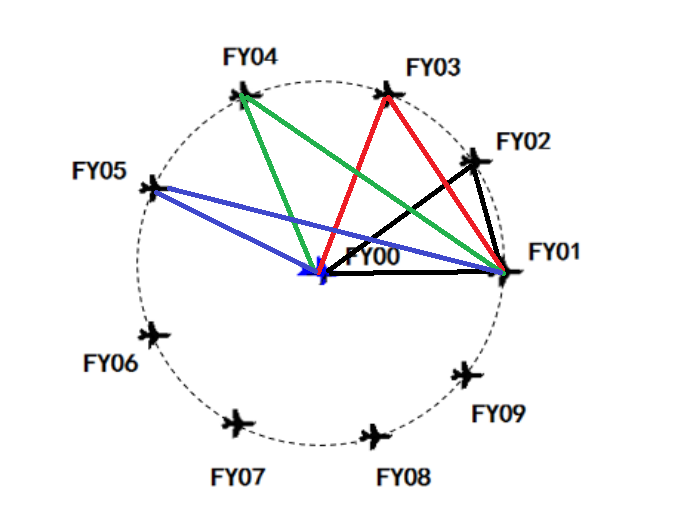
\includegraphics[width=0.6\textwidth]{pic1.png}
    \caption{发信机的位置情况} 
\end{figure}

由于太多的情况分类会导致模型的适用性有所下降,因此我们考虑不同的位置情况的通用描述量,即两架发信机与FY00形成的夹角。引入这个夹角作为模型的考虑变量,我们就将所有情况成功地在一个模型当中表达了出来。\\

2)接收机的位置关系

这里接收机的夹角取值范围是 $[0,\pi]$. 用 $\R^2$ 上的标准内积, 计算公式为
$$
    \angle BAC = \arccos (\frac{\langle A-B,A-C\rangle}{||A-B||_2||A-C||_2}),\quad A,B,C\in \R^2.
$$


\subsubsection{模型建立}

已知接收机与三架发射发信机形成的三个夹角, 接收机的位置可以被几乎唯一确定。
\begin{theorem}[定位基本定理]
    设 $O,A,B\in\R^2$ 互不相同, $\alpha,\beta,\gamma\in[0,\pi]$, 则满足 $\angle OCA = \alpha$, $\angle OCB = \beta$, $\angle BCA = \gamma$ 的点 $C$ 
    如果存在且不在过 $AOB$ 的圆上, 则 $C$ 能被唯一确定。
\end{theorem}
\begin{proof}
    满足 $\angle OCA = \alpha$ 的点 $C$ 的轨迹是圆弧或者直线. 考虑满足 $\angle OCA = \alpha$, $\angle OCB = \beta$ 的点 $C$. 
    利用 $OABC$ 不共圆, 这两个不重合圆弧
    或圆弧与直线或两条直线之间最多有两个交点. 若交点存在, 必有一个是 $O$, 而 $O$ 符合条件仅当 $\alpha=\beta=k\pi$. 
    此时 $O$ 是两直线的唯一交点. 否则, 符合条件的 $C$ 只可能为剩下一个交点或不存在. 
\end{proof}

若接收机机在理想位置附近,则接收机与三架发信机一定不共圆。接收机的位置就能被唯一确定。
通过引入发信机之间的夹角作为变量,我们考虑建立以下的基本数学模型:

\begin{figure}[H]
    \centering
    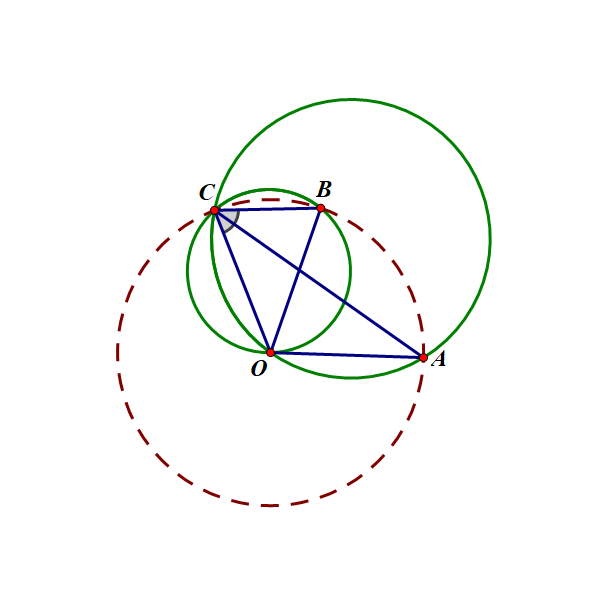
\includegraphics[width=0.5\textwidth]{sketch2}
    \caption{无人机定位系统的几何模型} 
\end{figure}

以 $O$ 为原点,$OA$ 为 $x$ 轴建立直角坐标平面,其中 $A$ 点的坐标为 $(r,0)$,$B$ 为另一架信号外机,设 $B$ 点的坐标为 $(rcos\theta,rsin\theta)$。同时,假设$\angle B C D = \beta$, $ \angle A C O = \alpha$。
由以上条件,得到 $AOC$ 的圆周方程:
$$
x ^ { 2 } + y ^ { 2 } - r x + \frac { r } { \tan \alpha } y = 0.
$$
同样,得到 $BOC$ 的圆周方程:
$$
x ^ { 2 } + y ^ { 2 } + ( - r \cos \theta - \frac { r \sin \theta } { \tan \beta } ) x + ( \frac { r \cos \theta } { \tan \beta } - r \sin \theta ) y = 0.
$$
利用两个圆弧的交点,我们得到 $C$ 点的坐标公式:
$$
x _ { c } = \frac { r A ^ { 2 } - r A / \tan \alpha } { A ^ { 2 } + 1 }, 
\quad y _ { c } = \frac { r A - r / \tan \alpha } { A ^ { 2 } + 1 }.
$$
其中:
$$
A = \frac { \frac { \cos \theta } { \tan \beta } - \sin \theta - \frac { 1 } { \tan \alpha } } { \cos \theta + \frac { \sin \theta } { \tan \beta } - 1 }.
$$

\subsubsection{模型求解}

通过基本的数学模型,我们设计算法对不同情况的点进行求解。考虑到接收机所处的位置不同,无法确定输入的角度的正负号,我们遍历一遍四种正负号的二元角度组,得到四个坐标定位。利用内积计算得到这四个坐标分别对应的三个夹角,与输入值比较,我们得以最终确定正确的坐标定位。于是,我们得到算法如下:

\begin{algorithm}[H]
\caption{\small 无人机定位算法}
\textbf{Input:} 接收的三个角度 $\alpha,\beta,\gamma$,两架信息外机的编号m,n,可接受误差限 $\delta$.\\
\textbf{Initialize:} $\theta=|m-n|\frac{2\pi}{9}$,$a^{(i)} = [\alpha,\alpha,-\alpha,-\alpha],b ^{(i)}= [\beta,-\beta,\beta,-\beta],O=(0,0),A=(1,0),B=(cos\theta,sin\theta),i=1$.\\
\textbf{Output:} 接收机的坐标 $(x,y)$ (单位为百米). \\
\textbf{Step1} 计算 $$N = \frac { \frac { \cos \theta } { \tan b^{(i)} } - \sin \theta - \frac { 1 } { \tan a^{(i)} } } { \cos \theta + \frac { \sin \theta } { \tan b^{(i)} } - 1 }.$$
\textbf{Step2} 计算 $$x= \frac { r N ^ { 2 } - r N / \tan a^{(i)} } { N ^ { 2 } + 1 } \quad y = \frac { r N - r / \tan ^{a(i)} } { N ^ { 2 } + 1 }\quad temp=(x,y).$$
\textbf{Step3} 计算 $$\alpha _ { t e m p } = \arccos ( \frac { ( temp  - A ) \cdot ( O - A ) } { | \operatorname temp - A | | O - A | } )$$ $$\beta _{ temp} = \arccos ( \frac { ( temp - B ) ( O - B ) } { | temp - B | | O - B | } )$$ $$\gamma_ { temp } = \arccos ( \frac { ( temp - A ) ( B - A ) } { |  temp - A | | B - A | } ).$$
\textbf{Step4} 如果存在 $|\alpha-\alpha_{temp}|\quad|\beta-\beta_{temp}|\quad|\gamma-\gamma_{temp}|$ 大于误差限 $\delta$, 则 $i=i+1$, 转至Step2, 直到满足误差限。
\end{algorithm}

\subsection{第二问:未知编号的无人机定位}
\subsubsection{小误差模型的建立与求解}
由于在不发生意外情况时,无人机相较于理想位置的偏差不会太大,因此我们首先考虑无人机的位置偏差足够小的情况。当在这个条件下,我们选择利用无人机的理想位置来确定无人机的编号。我们首先考虑三架无人机作为发信机的情况。通过理想位置的数据,我们计算出所有的角度信息三元组以及他们对应的发信机和接收机编号作为我们的信息库。

通过观察计算得到的三元组,我们发现,每个三元组都对应了至少两种发信机和接收机的编号情况,即两种不同的编号情况对应的接收信息完全相同,我们无法通过任何方式对它们进行区分。通过进一步计算四架及以上的发信机信息库,我们发现随着发信机数量的增加,同一个输入信息对应的编号情况也随之增加,无论选择几架发信机都无法对接收机进行有效定位。

为了解决这个问题,我们引入其他已知条件来增强我们的信息库:

1.接收机能够获取自己的编号信息。

2.接收机能够得知FY00和FY01对应形成的角度信息。

通过以上两个条件的限定,我们重新计算三架发信机形成的三元组$\{x^{i}\}$,并将FY00和FY01对应的角度信息放在三元组的第一位。获取输入信息$y$后,第一步,我们对比信息库当中的三元组和输入的角度信息三元组的第一位,即选择所有的$x^{(i)}$,满足:$$x ^ { ( i ) } = \operatorname { argmin } | x ^ { ( i ) }_1 - y_1 |$$

第二步,由于三个角度信息中,只有两个是独立的有效信息,因此我们删去所有三元组中最大的角度,防止冗余信息对模型的准确性产生未知的影响,最终生成信息库和输入信息对应的二元组。

第三步,我们通过计算范数来确定信息库当中和输入信息最接近的二元组,并结合接收机的编号,确定定位机的编号信息。由于范数的接近并不能够和距离的接近完全对等,因此我们考虑使用三种范数,即L1范数,L2范数和无穷范数,通过对比他们的正确率选择出合适的范数。

第四步,利用第一问的无人机定位算法,得到接收机的有效定位。

最终,我们得到完成的小误差定位算法如下:
\begin{algorithm}[H]
\caption{\small 小误差定位算法}
\textbf{Input:} 信息库$\{x^{(i)}\}$和对应的编号信息$\{m^{(i)}\}$,角度信息y,接收机编号n\\
\textbf{Output:} 接收机的有效定位\\
\textbf{Step1} 对所有$\{x^{i}\}$,筛选$x^{(i)}$满足$$x ^ { ( i ) } = \operatorname { argmin } | x ^ { ( i ) }_1 - y_1 |$$\\
\textbf{Step2} 对所有$\{x^{i}\}$,删除$$x _ { k } ^ { ( i ) } = \max ( x _ { j } ^ { ( i ) } ) \quad ( j = 1,2,3 )$$\\
\textbf{Step3} 选择$x^{(i)}$满足$$x ^ { ( i ) } = \operatorname { argmin } \| x ^ { ( i ) } - y \| _  { p }\quad ( p = 1,2 , \infty )$$\\
\textbf{Step4} 查找$x^{(i)}$对应的编号信息,同时满足$$m^{(i)}_2=n$$\\
\textbf{Step5} 调用无人机定位模型(Algorithm1)计算接收机位置\\
\end{algorithm}

利用小误差定位算法,我们得到三种范数在误差限20\%的情况下,各自的正确识别点和错误识别点,分别用红色和蓝色标出,模型结果如下图所示:

\begin{figure}[H]
    \centering
    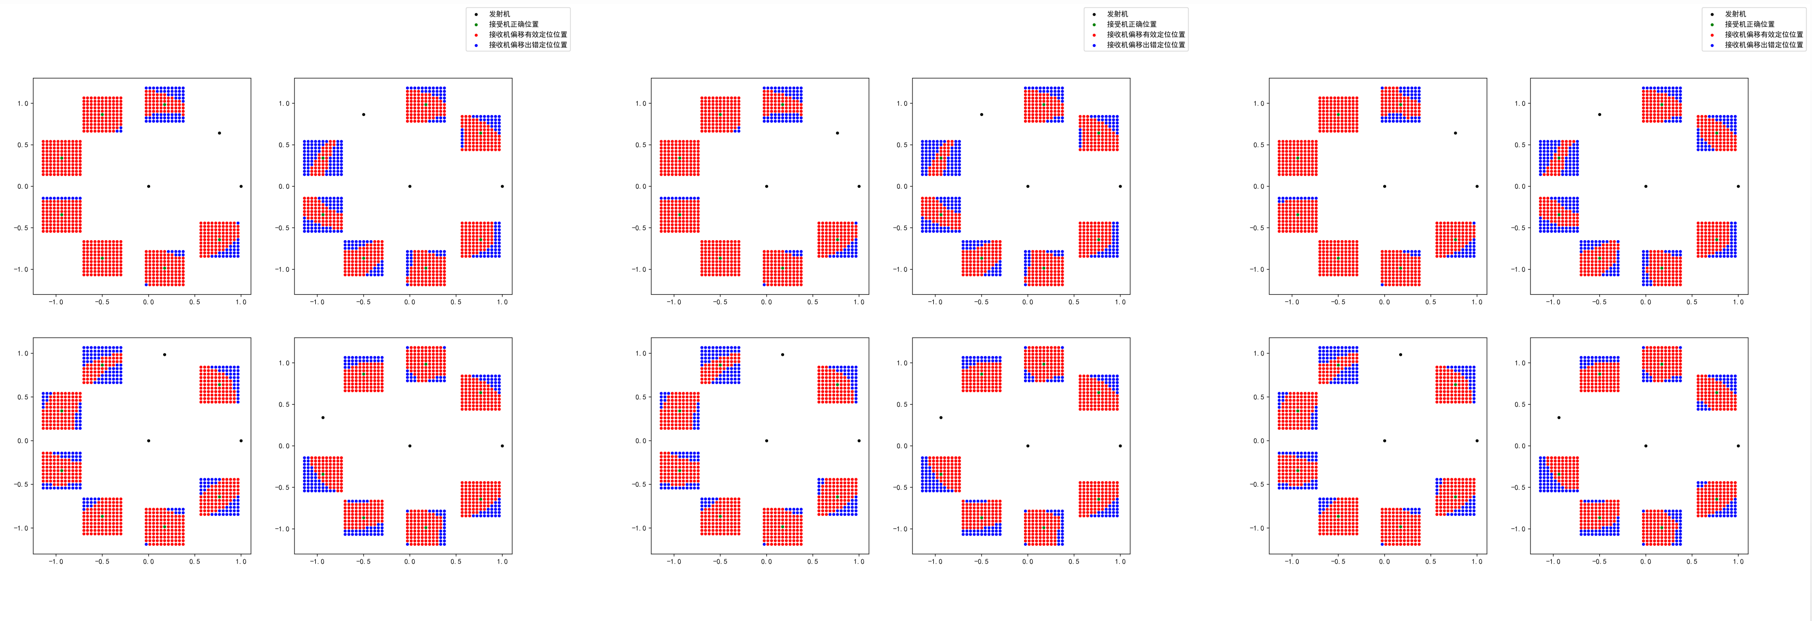
\includegraphics[width=1\textwidth]{two}
    \caption{基于不同范数的无人机定位} 
\end{figure}

通过观察结果我们发现,L1范数和L2范数的结果要好于无穷范数,并且三种范数都能在误差小于6\%,即误差足够小的情况下对接收机做出完全准确的定位,随着误差限的增加,仍然能够保持比较高的正确识别率。


\subsubsection{大误差模型的建立与求解}
当无人机没有误差限制的时候,我们完全无法确定发信机的编号,由于没有角度的限制,相同的输入信息对于每一种发信机组合都能够得到一个定位。并且由于角度信息的所属关系的不确定,随着发信机的数量增加,系统的混沌程度也随之上升,因此在无误差限制的情况下想要完全确定无人机的定位是不可能的。在这种情况下,我们希望尽可能增加正确判断无人机位置的范围基于无人机偏离理想位置过大的可能性较低的事实,我们引入一个新的条件,即无人机的可能位置以无人机的理想位置为中心,呈二维正态分布的随机状态。

在这样的条件下,我们认为无人机的实际位置接近自身的理想位置越近,概率越大,因此我们通过角度信息和所有包含FY00和FY01在内的三架发信机组合,计算出接收机实际位置可能的点位,通过计算这些点位和接收机理想位置的欧几里得范数,找到最接近理想位置的点位,并以这个点位作为无人机的有效定位。

以这个想法为基础,我们对其进行规范化和量化,得到大误差定位算法如下:
\begin{algorithm}[H]
\caption{\small 大误差定位算法}
\textbf{Input:} 接收到的角度信息y,接收机的编号k,接收机理想位置$q_0$\\
\textbf{Output:} 无人机的位置q\\
\textbf{Step1} 调用无人机定位算法(Algorithm1),对所有$j\in\{2,3,4,5,6,7,8,9\}$且$j\neq k$,以FY00,FY01,FY0j作为发信机计算无人机位置序列$\{q^{(j)}\}$\\
\textbf{Step2} 选择$q^{(j)}$满足$$q ^ { ( j ) } = argmin \| q_0 - q ^ { ( j ) } \| _ { 2 }$$ \\
\textbf{Step3} 决定$q^{(j)}$作为无人机的实际位置$$q= q ^ { ( j ) }$$
\end{algorithm}

\subsection{第三问模型的建立与求解}
    注意到理想情况下FY01,FY04,FY07构成一个等边三角形,FY00是它的中心。第一步我们将固定FY00和FY01,
    通过反复调整FY04和FY07,使得FY01,FY04,FY07构成以FY00为中心的等边三角形。下面的定理保证了这样
    调整进行得很快。
\begin{theorem}[等边三角形定理]
\label{dbsjx} 
    设 $O=(0,0)$, $C=(1,0)$,   
    $A^{(0)}=(1+\Delta,-\frac{2\pi}3-\delta)\in \R^{\geq 0}\times S^1$. 用如下递归的方式构造点列
    $\{B^{(i)}\}_{i\geq 1}$, $\{A^{(i)}\}_{i\geq 1}$: 
    $B^{(i)}=(r_B^{(i)},\theta_B^{(i)})$, $\theta_{B}^{(i)}\in (\frac \pi 2,\pi)$ 是
    第二象限中满足 $\angle CB^{(i)}O=\angle OB^{(i)}A^{(i-1)}=\frac\pi6$ 的点, 
    $A^{(i)}=(r_A^{(i)},-\theta_A^{(i)})$, $\theta_{A}^{(i)}\in (\frac \pi 2,\pi)$ 是
    第三象限中满足 $\angle CA^{(i)}O=\angle OA^{(i)}B^{(i)}=\frac\pi6$ 的点(接下来构造 $B^{(i+1)}$, $A^{(i+1)})$. 
    则 
    \begin{equation}
    \begin{aligned}
        r_A^{(i)}=1+o((|\Delta|+|\delta|)^{(i)}),\quad r_B^{(i)}=1+o((|\Delta|+|\delta|)^{(i-1)}),
        \\
        \theta_A^{(i)}=\frac{2\pi}{3}+o((|\Delta|+|\delta|)^{(i)}),\quad \theta_B^{(i)}=\frac{2\pi}{3}+o((|\Delta|+|\delta|)^{(i-1)}).
    \end{aligned}
    \label{1}
    \end{equation}
    利用有限维 Banach 空间的范数等价性, 有序列 $A^{(i)}$, $B^{(i)}$ 分别依2-范数超线性收敛到
    (converge superlinearly\cite{dennis1974characterization} under Euclidean norm to) $(1,\frac{-2\pi}3)$, $(1,\frac{2\pi}3)$.
\end{theorem} 

\begin{figure}[H]
    \centering
    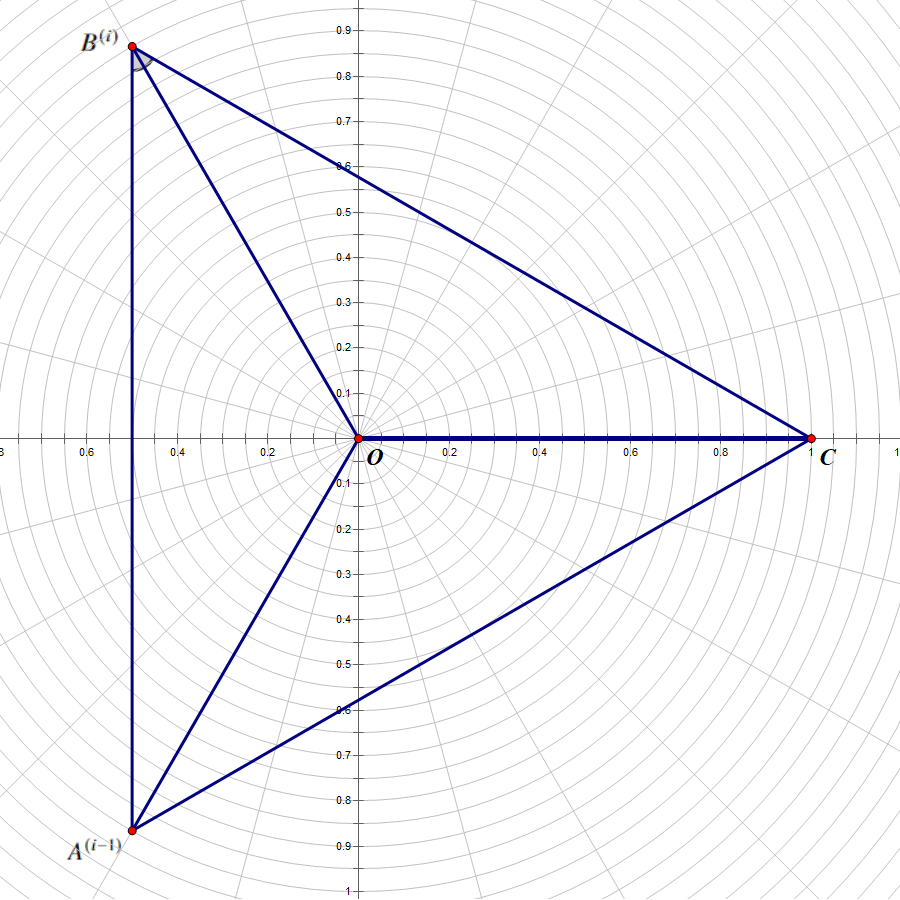
\includegraphics[width=0.5\textwidth]{sketch1}
    \caption{从 $A^{(i-1)}$ 构造 $B^{(i)}$ 的过程} 
\end{figure}

\begin{proof}
    不妨设 $r_A^{(i-1)}=1+\Delta_A^{(i-1)}$, $\theta_A^{(i-1)}=\frac{2\pi}{3}+\delta_A^{(i-1)}$. 根据几何关系,有 
    $$
    r_A^{i-1}\sin(\theta_B^{(i)}+\theta_A^{(i-1)}-\frac{7\pi}{6})=\sin(\frac{5\pi}{6}-\theta_{B}^{(i)})=\frac12 r_B^{(i)}.
    $$
    做 Taylor 展开,忽略一阶小就有
    $$
        \theta_{B}^{(i)}= \frac{2\pi}3-\frac{1}{2} \delta_A^{(i-1)}-\frac{\sqrt 3}6 \Delta_A^{(i-1)}+o(|\Delta_A^{(i-1)}|+|\delta_A^{(i-1)}|)
        ,\quad r_{B}^{(i)} = 1 +\frac{\sqrt3}{2} \delta_A^{(i-1)}+\frac12 \Delta_A^{(i-1)}+o((|\Delta_A^{(i-1)}|+|\delta_A^{(i-1)}|).
    $$
    利用旋转对称性,可得
    \begin{equation}
    \begin{aligned}
        \theta_{A}^{(i)}= \frac{2\pi}3-\frac{1}{2} (-\frac{1}{2} \delta_A^{(i-1)}-\frac{\sqrt 3}6 \Delta_A^{(i-1)})
        -\frac{\sqrt 3}6 (\frac{\sqrt3}{2} \delta_A^{(i-1)}+\frac12 \Delta_A^{(i-1)}) +o(|\Delta_A^{(i-1)}|+|\delta_A^{(i-1)}|)
        \\=o(|\Delta_A^{(i-1)}|+|\delta_A^{(i-1)}|).&
    \end{aligned}
    \label{2}
    \end{equation}
    同理 $r_{A}^{(i)}=o(|\Delta_A^{(i-1)}|+|\delta_A^{(i-1)}|).$ 利用数学归纳法可得结果. 
\end{proof}

    利用调整两个夹角为 $\frac\pi6$ 的方式,上面的定理保证了 FY04 和 FY07 能被快速地调整到理想位置。
    接下来我们假定 FY04 和 FY07 的位置正确,通过第一小问的方法即可定位所有其他飞机并调整他们到理想位置。

\begin{algorithm}[H]
    \caption{\small 无人机位置调整算法}
    \textbf{Input:} 预计无人机位置与理想位置的径向绝对误差 $\Delta$, 角向绝对误差 $\delta$, 可接受误差限 $\delta_0$.\\
    \textbf{Initialize:}. $r=1$.\\
    \textbf{Output:}. 无人机的正确位置.\\
    \textbf{Step1} 调整 FY04 的位置, 使得 FY04接收到的角度信息为 $\frac{\pi}{6}$,$\frac{\pi}{6}$,$\frac{\pi}{3}$.\\
    \textbf{Step2} 调整 FY07 的位置, 使得 FY07接收到的角度信息为 $\frac{\pi}{6}$,$\frac{\pi}{6}$,$\frac{\pi}{3}$.\\
    \textbf{Step3} 如果$(|\Delta|+|\delta|)^r\geq\delta_0$,回到 Step1,$r=r+1$,直到满足可接受误差限.\\
    \textbf{Step4} 对 $j\in\{2,3,5,6,8,9\}$, 计算 FY0j 在理想位置相对于 FY07, FY00, FY01 的夹角,并调整 FY0j 使得它与 FY07, FY00, FY01 的夹角与理想情况一致.\\
\end{algorithm}

\subsection{问题二:无人机编队的调整}

\subsubsection{模型建立}
第三问的算法提供了一种调整位置的优秀方案,只要无人机队形中能找到一个接近等边三角形和它的中心的四架飞机,就可以很快地
将他们调整到合适的位置,以便其他飞机参照。因此对于飞机队形的调整问题,我们仍延续上一问的思路。

首先固定三架发信机 $A$, $O$, $B$, 接收机 $C$ 按照 $COB$ 
都处于理想位置时计算得到的理想角度进行调整。由于我们仅考虑相对角度和距离,不妨设 $O$, $C$ 处于理想位置。
考虑到 $B$ 可能有偏差, 此时 $A$ 与理想位置之间也会有些许偏差。
然后再用同样的方法调整 $A$ 的位置,此时 $BOC$ 作为发信机。如此重复下去相互调整 $B$, $A$ 位置。下面的定理保证了
只要 $B$, $C$ 的初始位置接近理想位置,且四架飞机之间的位置关系满足一定条件,这样的调整方案是收敛的。此外,
定理还给出了快速收敛时四架飞机位置需要满足的条件。定理可以自然地推出等边三角形定理。
这个定理有一定的技术性,在此省略了部分计算过程,但是其证明思想与等边三角形定理一致。 
\begin{theorem}[三角形内点调整法收敛判据]
    \label{remarkable}
    设 $O=(0,0)$, $C=(1,0)$. 取 $A_0=(r_A, -\theta_A)$, $B_0 = (r_B,\theta_B)$ 为目标位置, 点 $O$ 位于
    三角形 $A_0B_0C$ 的内部.
    固定 $\angle OCB_0=\alpha_1$, $\angle OCA_0=\beta_1$, $\angle OB_0A_0=\alpha_2$, $\angle OB_0C=\beta_2$,
    $\angle OA_0C=\alpha_3$, $\angle OA_0B_0=\beta_3$,  
    用如下递归的方式构造点列 $\{B^{(i)}\}_{i\geq 1}$, $\{A^{(i)}\}_{i\geq 1}$: 先找到
    $B^{(i)}=(r_B^{(i)},\theta_B^{(i)})$ 满足 $\angle A^{(i-1)}B^{(i)}O=\alpha_2, \angle CB^{(i)}O=\beta_2$, 再找到
    $A^{(i)}=(r_A^{(i)},-\theta_A^{(i)})$, 满足 $\angle CA^{(i)}O=\alpha_3, \angle OA^{(i)}B^{(i)}=\beta_3$. 如此重复下去.
    设 
    $$
        Z = \frac{(\cot \beta_3-\cot\beta_1)(\cot \alpha_2-\cot \alpha_1)}
        {(\cot \alpha_1+\cot \beta_3)(\cot \alpha_2+\cot \beta_1)}.
    $$
    若 $|Z|< 1$ 则点列 $A^{(i)}$, $B^{(i)}$ 线性收敛(linearly convergent)到 $A_0$, $B_0$. 
    该收敛是超线性 (superlinear) 的当且仅当 $\alpha_2=\alpha_1$ 或 $\beta_3=\beta_1$. 
\end{theorem}
\begin{figure}[H]
    \centering
    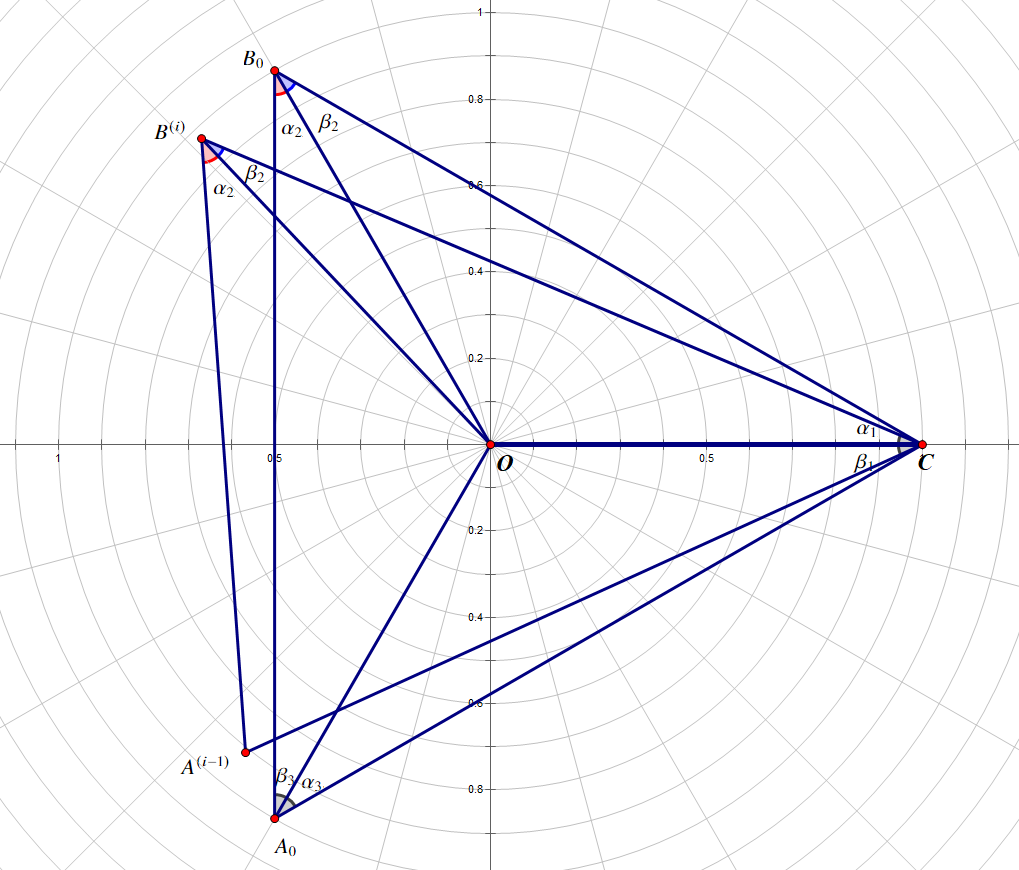
\includegraphics[width=0.6\textwidth]{sketch4}
    \caption{从 $A^{(i-1)}$ 构造 $B^{(i)}$ 的过程} 
\end{figure}
\begin{proof}
    这个定理是等边三角形定理的推广. 根据几何关系, 有
    $$
        \frac{1}{\sin\beta_2}=\frac{r_B^{(i)}}{\sin(\alpha_1+\theta_B-\theta_B^{(i)})},\quad
        \frac{r_A^{(i-1)}}{\sin\alpha_2} = \frac{r_B^{(i)}}{\sin(\beta_3-\theta_B+\theta_B^{(i)}-\theta_A+\theta_A^{(i-1)})}.
    $$
    做 Taylor 展开, 忽略高阶小, 有
    $$
        \theta_B^{(i)}-\theta_B = \frac{-\cot \alpha_2}{\cot\beta_3+\cot\alpha_1}(\theta_A^{(i-1)}-\theta_A)+
        \frac{-1}{\cot\beta_3+\cot\alpha_1}(r_A^{(i-1)}-r_A)+o(|\theta_A^{(i-1)}-\theta_A|+|r_A^{(i-1)}-r_A|),
    $$
    且 
    $$
        r_B^{(i)}-r_B= -\cot\alpha_1(\theta_B^{(i)}-\theta_B)+ o(|\theta_A^{(i-1)}-\theta_A|+|r_A^{(i-1)}-r_A|).
    $$
    设 
    $$
    X=\frac{\cot \beta_3(\cot \alpha_2-\cot \alpha_1)}
    {(\cot \alpha_1+\cot \beta_3)(\cot \alpha_2+\cot \beta_1)},\quad
    Y=\frac{(\cot \alpha_2-\cot \alpha_1)}
    {(\cot \alpha_1+\cot \beta_3)(\cot \alpha_2+\cot \beta_1)}.
    $$
    代入上一步的误差项迭代, 就有
    $$
    \theta_A^{(i)}-\theta_A = X(\theta_A^{(i-1)}-\theta_A) + Y(r_A^{(i-1)}-r_A) + o(|\theta_A^{(i-1)}-\theta_A|+|r_A^{(i-1)}-r_A|).
    $$
    和
    $$
    r_A^{(i)}-r_A= -\cot\beta_1X(\theta_A^{(i-1)}-\theta_A)-\cot\beta_1Y(r_A^{(i-1)}-r_A)+ o(|\theta_A^{(i-1)}-\theta_A|+|r_A^{(i-1)}-r_A|).
    $$
    写成矩阵形式, 就有
    $$
        \begin{pmatrix}
            \theta_A^{(i)}-\theta_A\\
            r_A^{(i)}-r_A
        \end{pmatrix}
        =
        M
        \begin{pmatrix}
            \theta_A^{(i-1)}-\theta_A\\
            r_A^{(i-1)}-r_A
        \end{pmatrix},
        \quad
        M=
        \begin{pmatrix}
            X&Y\\
            -\cot\alpha_2 X& -\cot\alpha_2 Y\\
        \end{pmatrix}
        +o(|\theta_A^{(i-1)}-\theta_A|+|r_A^{(i-1)}-r_A|).
    $$
    因为 $\sigma_M=\{0, X-\cot\beta_1 Y\}$ ( $\sigma_M$ 表示矩阵 $M$ 的谱), 令 $Z=X-\cot\beta_1Y$. 
    若 $|Z|<1$, 则点列 $A^{(i)}$, $B^{(i)}$ 线性收敛(linearly convergent)到 $A_0$, $B_0$. 
    该收敛是超线性 (superlinear) 的当且仅当 $\alpha_2=\alpha_1$ 或 $\beta_3=\beta_1$. 
\end{proof}

    对于给定的飞机队形,我们首先找到满足定理条件的四架飞机,用定理给出的方式调整位置。进行足够多次迭代后,再利用调整好的飞机确定其他飞机的位置。
    下面笔者给出一些满足 $\alpha_1=\alpha_2$ 或 $\beta_1=\beta_3$ 的图形。可以发现,在一般的规则队形中,这样的图形是常见的,例如题目中给出的锥形编队。
    如果找不到这样的图形,我们可以找到 $|Z|$ 最小即收敛速度最快的调整方法。
%----------- 六、模型的分析与检验 ----------
\section{六、模型检验与灵敏度分析}
\subsection{第一问的模型检验}
我们设计相应的测试对我们的算法模型进行测试以验证算法的正确性。测试方案如下:

对于发送机不同夹角的4种情况进行测试模拟。选定R = 1。每次测验通过计算机随机选定一台编号的接收机,我们认为他的位置距离他的理想位置至多有ErrorRate的误差。通过坐标的计算,程序会给接收机提供三个发信机的三个角度信息来模拟真实场景,接收机得到该角度信息后,通过第一问得到的算法,算出自身的x轴坐标以及y轴坐标,与计算机选定的真实坐标进行比对,如果两者的差值小于误差$(10^{-5})$,我们认为这次定位正确的,红点是能够准确定位的点,而蓝点则表示定位失败。重复上述测验100次,计算出程序定位的错误率。\\
测试结果如下图显示(ErrorRate=20\%):
\begin{figure}[H]
    \centering
    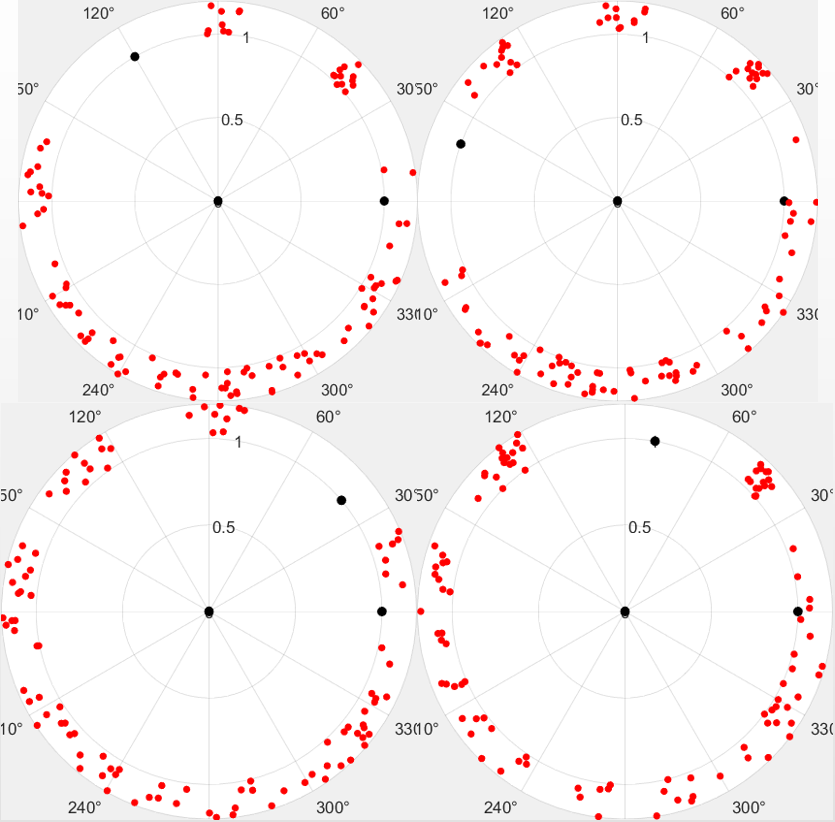
\includegraphics[width=0.6\textwidth]{check1}
    \caption{第一问模型结果} 
\end{figure}

上图为ErrorRate=20\%的测试图,红色的点是随机测试能够正确定位的点,黑色的是发射机,他的位置没有偏差。由于情况是对称的,因此4种情况便能模拟所有可能的情形。通过结果检验,我们的模型在20\%的误差限时能够完全定位无人机的位置。我们接着改变误差率ErrRate,当增大误差范围的时候,除开接收机与两台无人机形成三点一线的特殊情形,我们的模型都能够对无人机做出正确的定位。因此我们认为定位算法是有效的。\\
附件中Corrdinate.m代码是定位算法,接受四个对应角的输入能够得到该点的x,y坐标。Angle为计算三点夹角的辅助函数。test.m是具体的测试模拟算法,测试4种情形,每种情形测试100次并且以“发送机编号-正确次数.png”的格式保存图片到本地。

\subsection{第二问的模型检验}
\subsection{第三问的模型检验}
\subsection{问题二的模型检验}

\section{七、模型的评价、改进与推广}
\subsection{模型的优点}
优缺点是必须要写的内容,改进和推广是可选的,但还是建议大家写,实力比较强的建模者可以在这一块充分发挥,这部分对于整个论文的作用在于画龙点睛。
\subsection{模型的缺点}
缺点写的个数要比优点少
\subsection{模型的改进}
主要是针对模型中缺点有哪些可以改进的地方\cite{risken1996fokker};
\subsection{模型的推广}
将原题的要求进行扩展\cite{rossler1979equation},进一步讨论模型的实用性和可行性\cite{mckean1970nagumo}。

%----------- 参考文献 ----------
\bibliographystyle{unsrt} %规定了参考文献的格式
\begin{center}
\bibliography{reference} %调出LaTeX生成参考文献列表
\end{center}
\textcolor{red}{(所有引用他人或公开资料(包括网上资料)的成果必须按照科技论文的规范列出参考文献,并在正文引用处予以标注。}

\textcolor{red}{常见的三种参考文献的表达方式(标准不唯一):
书籍的表述方式为: [编号] 作者,书名,出版地:出版社,出版年月。
期刊杂志论文的表述方式为: [编号] 作者,论文名,杂志名,卷期号:起止页码,出版年。
网上资源(例如数据库、政府报告)的表述方式为: [编号] 作者,资源标题,网址,访问时间。)}
%----------- 附录 ----------
\newpage
\section{附录}

\begin{table}[htbp]
    \centering
    \begin{tabular}{|p{14.0cm}|}
 %指定单元格宽度, 并且水平居中。
    \hline
    \textbf{附录1} \\ %换行 
    \hline
    介绍:支撑材料的文件列表  \\ 
    \\
    \\
    \\
    \hline
    \end{tabular}
\end{table}

\begin{table}[htbp]
    \centering
    \begin{tabular}{|p{14.0cm}|}
 %指定单元格宽度, 并且水平居中。
    \hline
    \textbf{附录2} \\ %换行 
    \hline
    介绍:该代码是某某语言编写的,作用是什么   \\ 
    \\
    \\
    \\
    \hline
    \end{tabular}
\end{table}

除了支撑材料的文件列表和源程序代码外,附录中还可以包括下面内容:
\begin{itemize}
\item 某一问题的详细证明或求解过程;
\item 自己在网上找到的数据;
\item 比较大的流程图;
\item 较繁杂的图表或计算结果
\end{itemize}

\end{document}